\section{Experimental Results}
\label{sec:expResults}
%Results should be clearly displayed and should provide a suitable representation of your results for the points you wish to make. Graphs should be labeled in a legible font and if more than one result is displayed on the same graph then these should be clearly marked.   Please choose carefully rather than presenting every results. Too much information is hard to read and often hides the key information you wish to present. Make use of statistical methods when presenting results, where possible to strengthen the results.  Further, the format of the presentation of results should be chosen based on what issues in the results you wish to highlight. You may wish to present a subset in the experimental section and provide additional results in the appendix.

\subsection{Parameter Settings}
\label{subsec:parameterSettings_results}

Table \vref{table:parameterSettings2} shows the parameters tested, their candidate values and the selected value. The complete experimental steps with the corresponding results can be found in, Appendix \ref{appendixC}, Table \vref{table:pm1} and Table \vref{table:pm2}. 

    \begin{table}[H]
    \centering
    \begin{tabular}{|c|c||c|}
    \hline
    Parameters & Candidate values & Selected value\\
    \hline
    $s$ & 10, 25, 50, 100, 150 & 50$^*$ \\
    $i$ & 1, 10 , 50, 100, 125 & 100$^*$ \\
    $E$ & 1\%, 10\%, 25\% 50\%, 75\%, 90\%, 99\% & 50\% \\
    $p_{b}$ & 0.0, 0.1, 0.3, 0.5, 0.7, 0.9 & 0.9 \\
    $AF$ & 0\%, 1\%, 5\%, 10\%, 50\%, 75\%, 100\% & 25\% \\
    $CA$ & 0\%, 1\%, 5\%, 10\%, 50\%, 75\%, 100\% & 5\% \\
    \hline
    \end{tabular}
    \caption {Results from the Parameter Settings Experiment}
    \begin{itemize}[noitemsep]
    \item[$^*$:]  Selected value is based on results presented in Figure \vref{fig:svsitesting} and Figure \vref{fig:svsiruntime} 
    \end{itemize}
    \label{table:parameterSettings2}
    \end{table}
    

\textbf{Evaluation}
\newline
Based on the results shown i Appendix \ref{appendixC}, Table \vref{table:pm1} and Table \vref{table:pm2}, we observe that the stated Confidence Interval does not become remarkably better by running the algorithm 50 times compared to 30. This makes it reasonable to conclude that the results regarding the parameters that were ran 30 times are valid. 
\newline
%Because our confidence coefficient is sat to correspond to 95\%, we are able to say that we are 95\% confident that the true population parameter is between the lower and upper calculated values.

Based on Table \vref{table:pm1} we see that the selected value for parameters $s$ and $i$ are sat to respectively 150 and 100 based on the average $ATT$ and the average $TOTFIT$. However, one thing that is not considered in the initial parameter setting experiment is that the size of $s$ and $i$ affects each other. A colony of 10 ants ran 100 times would produce similar results to 100 ants ran 10 times. Because of this additional tests are performed with respectively a colony size ($s$) of 50, 75, 100, 125 and 150 each ran with 100 iterations ($i$). The results of these tests are presented in Figure \vref{fig:svsitesting}. Table \vref{table:pm1} in Appendix \ref{appendixC} shows that a $s$ below 50 sometimes produced ant colonies were no ants satisfy the initial Constraint \ref{itm:criteriaConnectedGraph} described in Section \vref{sec:algoConstraints}. When $s$ is 10, this occurs on average 16\% of the iterations and when the swarm size is 25 i occurs on average 0.5\% of the iterations. The reader recalls from Section \vref{sec:algoEvaluation} that if no ant satisfy the initial constraint, no ant is either evaluated, and the iteration therefor becomes invalid. Especially when $s$ is 10, this leads to that in practice the algorithm is ran less iterations than the sat $i$. 

\begin{figure}[H]
\begin{center}
  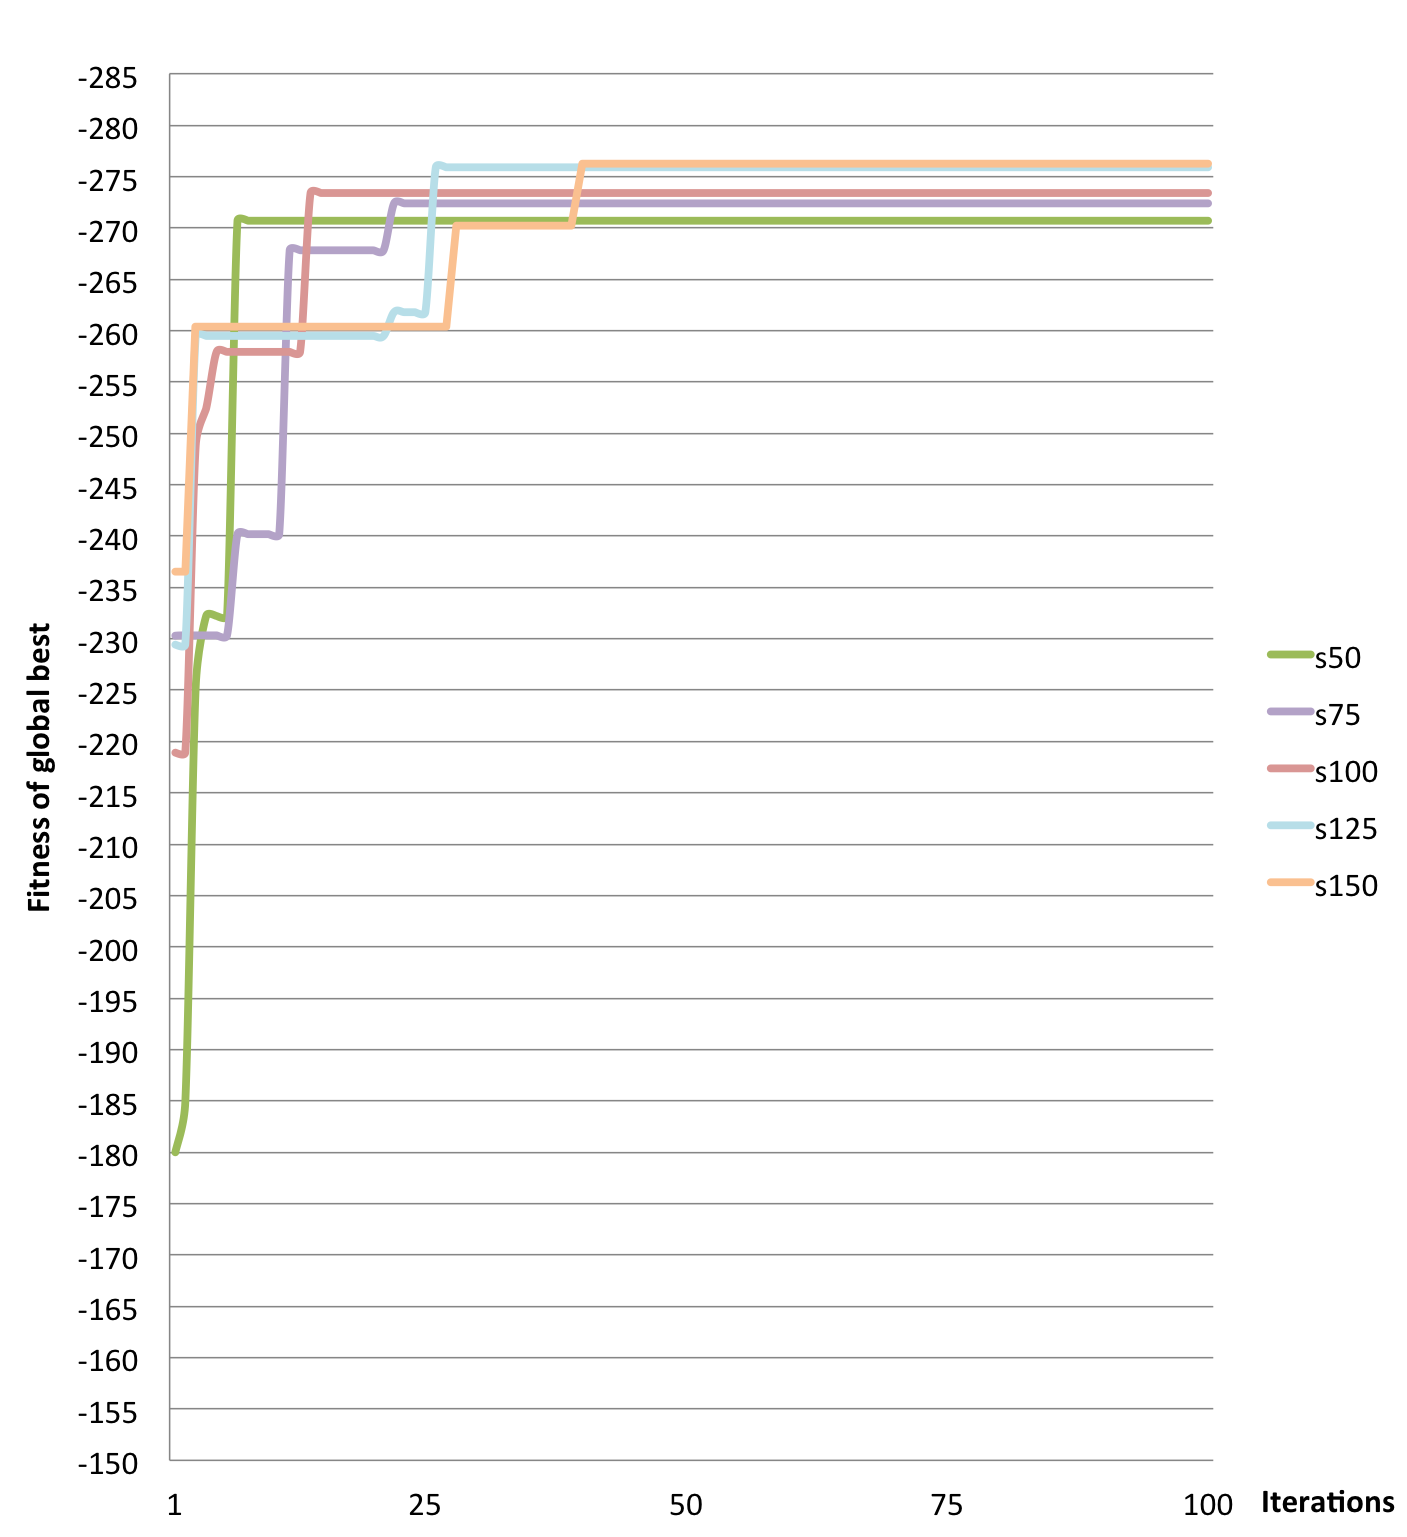
\includegraphics[width=4in]{assets/svsitest.png}
  \end{center}
  \caption{Evolution of Global Best Total Fitness ($TOTFIT$)}
  \label{fig:svsitesting} 
\end{figure}

Figure \vref{fig:svsitesting} shows the evaluation of the total fitness ($TOTFIT$) of the global best ant with the colony sizes mentioned above. The algorithm is run one time for each swarm size, and the $TOTFIT$ value is recorded for each iteration. As one can see from Figure \vref{fig:svsitesting} increasing the size of the colony leads to a better $TOTFIT$ value in both the initial and final iterations.  %In the first iteration, all edge values are zero, and the first point in the graph represents the $TOTFIT$ value after the first iteration. 

However, there is a great difference in the running time when increasing the colony size. Figure \vref{fig:svsiruntime} shows the respective run times in second. As one can see there is a big difference in running time with 125 ants compared to 100. Between 50 and 100 ants the running time increases with about 750 seconds, while between 100 and 125 the running time increases with about 1200 seconds. 

\begin{figure}[H]
\begin{center}
  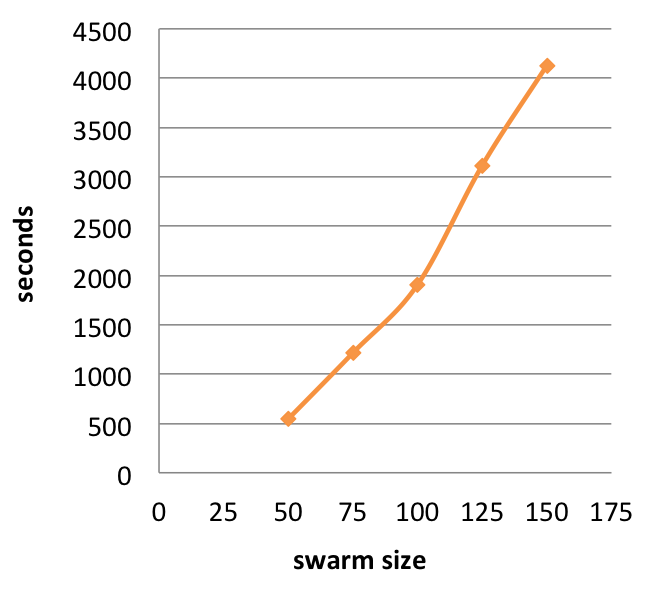
\includegraphics[width=2.5in]{assets/svsiruntime.png}
  \end{center}
  \caption{Evolution of the runtime, in seconds, in accordance to the swarm size}
  \label{fig:svsiruntime} 
\end{figure}

Because the algorithm is going to be run an excessive amount of times when testing performance, the selected value of parameter $s$ is sat to \textit{100}. This is done, even though both a $s$ of both 125 and 150 gave a better $TOTFIT$, due to the large difference in run time. 

As one can see from Figure \vref{fig:svsitesting}, the algorithm seems to converge before 50 iterations, regardless of the colony size. This also corresponds to our initial parameter testing of $i$, which only shows a small improvement of the average $TOTFIT$ and the average travel time $ATT$ of 100 iterations compared to 50. The run time also increases drastically with 100 iterations compared to 50. The algorithm uses 499 seconds on the first 50 iterations, while it uses 1408 seconds on the last 50 iterations. These reasons combined makes the selected value of parameter $i$ \textit{50} and not 100, even tough 100 produced slightly better results in the initial parameter setting experiment.

Observing the produced results of parameter $E$ in Table \vref{table:pm1}, evaporating 50\% of the pheromone each iteration gave the best average total fitness and the second best average travel time. Evaporating 75\% gave the best average travel time, and the second best total fitness, but according to the formula described in Section \vref{subsec:parameterSettings_setup} 50\% is selected. As one can observe, the best produced results is achieved by a candidate value greater or equal to 50\%. The algorithm seems to benefit from the fact that a great amount of pheromone evaporates each iteration. We believe this is because it compensates for some of the randomness the parameter $CA$ produces, by quickly removing pheromone from edges that were once used, but later discarded. One can also observe that the worst results were achieved when $E$ was sat to 99\%. Even though the algorithm benefits from a large percentage of evaporated pheromones, it reaches a threshold were the percentage becomes too big. By removing 99\% of the pheromone an edge that is usually used a lot, but for some reason not used as much the given iteration, it is ``punished'' too hard. 
\newline

The amount of $AF$ determines the amount of Following Ants ($FA$) in the next iteration, and the $FA$ follow the same path as the best ants' paths unconditionally. Observing the results obtained in Table \vref{table:pm2}, the $TOTFIT$ value deteriorates when the amount of $AF$ becomes greater than 25\%. When the amount of $FA$ becomes too great, a relatively large number of normal ants will not be able to explore new (possibly better) routes in the next iterations, and the algorithm may suffer from a local optima. But as one also can see, 25\% computes better results than the candidate values below. Rewarding some good route sets seems to boost the algorithms performance to some degree, and 25\% is selected as the final parameter for $AF$.

Based on the produced results, the selected value of parameter $p_b$ is 0.9. The value of $p_b$ is strongly dependent on the value of $AF$, because the more following ants, the more pheromone added to each edge in the best route sets. To ensure that rewarding more edges with the selected amount of pheromone did not negatively affect the algorithm's performance, the value of $p_b$ was tested with the new selected value of $AF$. As one can observe in Table \vref{table:pb_testing}, both $TOTFIT$ values have increased with the new increased value of $AF$, and the selected value for $p_b$ does not compute worse than when the $AF$ value was 10\%. The $ATT$ value increases after the new value of $p_b$, and the value of $p_b$ will be the same as it initial was selected. 

    \begin{table}[H]
    \centering
    \begin{tabular}{|c|c||c|c|}
    \hline
    $AF$ & $p_b$ & $ATT$ & $TOTFIT$\\
    \hline
    10\% & 0.5 & 11.302 & -269.279 \\
    10\% & 0.9 & 11.314 & -269.631 \\
    25\% & 0.5 & 11.366 & -272.392 \\
    25\% & 0.9 & 11.314 & -271.524 \\
    \hline
    \end{tabular}
    \caption {Testing the value of parameter $p_b$ to the parameter $AF$}
    \label{table:pb_testing}
    \end{table}

The value of $CA$ is sat to 5\% based on the results shown in Table \vref{table:pm2} in Appendix \ref{appendixC}. The reader recalls from Section \vref{sec:algoInitialization} that this means that there is a 5\% probability that an ant is declared ``crazy'' and thus makes completely random decisions. The results in Table \vref{table:pm2} shows that the algorithm benefits from the fact that some ants are declared crazy, but also that if the probability is greater than 25\%, both the average $ATT$ and the average $TOTFIT$ results become worse. This is not very surprising, because if half of the colony or more acts randomly, the algorithm looses some of the performing boosting features from ACO, such as favoring edges frequently walked by other ants. Like for $s$ below 50, a value of $CA$ above 50\% sometimes produces ant colonies were no ants satisfy the initial Constraint \ref{itm:criteriaConnectedGraph} described in Section \vref{sec:algoConstraints}. This is again not very surprising, because when such a large part of the colony acts randomly, several (and sometimes all) of these ants will create route sets that do not include every node in the network. The probability of creating a route set that does not contain all nodes are decreased in ``normal'' ants by the fact that they favor nodes they have not yet visited in the given route set. 


